\section{Method}
%
Next, we formulate the target task and describe the training data generation and representation learning. 
An overview of the proposed generation process is shown in \cref{fig:overview}.

\subsection{Task formulation}
%
The target task is instance-level image retrieval.
Given a query image, the goal is to retrieve all positive images from a database (db), \ie those that depict the same object instance as the query.
Images depicting different object instances, even if they belong to the same semantic category, are negatives and should not be retrieved.
This is an open-world task, testing on unseen objects from a variety of domains which may be seen or unseen during training.

We consider the efficient retrieval variant using global descriptors.  
Formally, an image $x$ is mapped to a $d$-dimensional global descriptor $\mathbf{z} = f_\theta(x) \in \mathbb{R}^d$.  
Retrieval is performed via nearest neighbor search in Euclidean space, ranking database descriptors based on their cosine similarity to the query.  
The encoder, parameterized by $\theta$, is optimized during training.
We focus on fine-tuning foundational models~\citep{zhai2023sigmoid} that already perform well by pretraining.  

\begin{figure*}[t]
% \vspace{5pt}
\centering
\includegraphics[width=.95\linewidth]{fig/overview.pdf}
% \vspace{-5pt}
\caption{Overview of instance-level training data generation.
A domain name or description is the only input, which is used to prompt an LLM to provide a list of object category names. 
Then, we generate examples of those categories using a GDM, remove the background, and synthesize lighting and background multiple times per generated example to create a diverse set of positive images for each instance.
} 
\label{fig:overview}
\end{figure*}

\subsection{Instance-level training data generation}
%
We propose a pipeline that requires only the name, or a textual description, of a target domain as input, and automatically generates an image training set with instance-level labels.
The process consists of four stages:
(i) \textit{Objects categories generation} by prompting an LLM to provide a list of %useful 
object category names;
(ii) \textit{Object instance generation} by prompting a GDM to generate object instances from each category;
(iii) \textit{Background generation} by synthesizing diverse backgrounds per instance;
(iv) \textit{Viewpoint variations} by augmenting the generated images with geometric transformations.
Each stage of the process is detailed below.

\paragraph{Object categories generation}
%
Object categories (\eg \textit{table}, \textit{chair}, \textit{clock}) are needed to prompt the GDM for image generation. 
We automatically obtain a list of object categories by prompting an LLM with minimal information about the domain of interest. 
In the general case in which we do not target a specific domain, the prompt we use is 
``\emph{Provide a raw list of names of everyday objects.}''
For specific domains, such as artwork, landmark, or product, we enrich the prompt with relevant information and hint with a few examples of object categories. 
Full details of the designed prompts are provided in the supplementary material. 
This approach yields a rich and diverse list of $C$ object categories.
Examples of category names generated for the general case are \textit{sofa}, \textit{desk}, while for the specific domains are \textit{bust}, \textit{castle}, and \textit{polaroid film}, for artwork, landmark, and product, respectively.

\paragraph{Object instance generation}
%
We prompt a GDM, in particular Stable Diffusion Turbo~\citep{sauer2025adversarial}, with an object category to generate $K$ images per category.
We assume that generating images with different random seeds produces variations that are distinct and recognizable as separate instances within the same category. 
Therefore, following an instance-level class definition, each of the $M$ generated images, where $M = C K$, is treated as a separate class in our training set.
To facilitate the follow-up step of background generation, we target a simple or uniform background. To achieve this, we add ``\emph{in a clean background}" to the prompt after the object category as in, ``\textit{a table in a clean background}." 
%
Examples in \cref{fig:sdimages} show that, even though the background removal process may fail in both cases, it is less likely to happen with the extended prompt, while the original prompt provides outputs with richer background.


\begin{figure*}[t]
\begin{center}    
% \vspace{5pt}
\footnotesize
\newcommand{\figclean}[2]{\includegraphics[width=42pt,height=42pt]{fig/sd/#1/clean/#2.png}&\includegraphics[width=42pt,height=42pt]{fig/sd/#1/clean/#2_fg.png}}
\newcommand{\figunclean}[2]{\includegraphics[width=42pt,height=42pt]{fig/sd/#1/unclean/#2.png}&\includegraphics[width=42pt,height=42pt]{fig/sd/#1/unclean/#2_fg.png}}
% \begin{tabular}{lcccccccc}
%                                         & sofa & sofa & lamp & X & X & X & X & X \\
% \raisebox{15pt}{SD - clean}  			& \includegraphics[width=42pt,height=42pt]{fig/sd/clean/sofa/0.png}					& \includegraphics[width=42pt,height=42pt]{fig/sd/clean/sofa/7.png} 			& \includegraphics[width=42pt,height=42pt]{fig/sd/clean/lamp/8.png} 			& \includegraphics[width=42pt,height=42pt]{fig/sd/clean/lamp/8.png} 				& \includegraphics[width=42pt,height=42pt]{fig/sd/clean/lamp/8.png} 		   & \includegraphics[width=42pt,height=42pt]{fig/sd/clean/lamp/8.png} 				  & \includegraphics[width=42pt,height=42pt]{fig/sd/clean/lamp/8.png} 		     & \includegraphics[width=42pt,height=42pt]{fig/sd/clean/lamp/8.png} 				 \\
% \raisebox{15pt}{bg. removal}           	& \includegraphics[width=42pt,height=42pt]{fig/sd/clean/sofa_rmv/fg_00360.png}  	& \includegraphics[width=42pt,height=42pt]{fig/sd/clean/sofa_rmv/fg_00388.png}  & \includegraphics[width=42pt,height=42pt]{fig/sd/clean/lamp_rmv/fg_32112.png}  & \includegraphics[width=42pt,height=42pt]{fig/sd/clean/lamp_rmv/fg_32112.png} 		& \includegraphics[width=42pt,height=42pt]{fig/sd/clean/lamp_rmv/fg_32112.png} & \includegraphics[width=42pt,height=42pt]{fig/sd/clean/lamp_rmv/fg_32112.png}  	  & \includegraphics[width=42pt,height=42pt]{fig/sd/clean/lamp_rmv/fg_32112.png} & \includegraphics[width=42pt,height=42pt]{fig/sd/clean/lamp_rmv/fg_32112.png}  	 \\
% \raisebox{15pt}{SD - not clean}      	& \includegraphics[width=42pt,height=42pt]{fig/sd/noclean/sofa/1.png}				& \includegraphics[width=42pt,height=42pt]{fig/sd/noclean/sofa/1.png}           & \includegraphics[width=42pt,height=42pt]{fig/sd/noclean/lamp/8.png} 			& \includegraphics[width=42pt,height=42pt]{fig/sd/noclean/lamp/8.png}  				& \includegraphics[width=42pt,height=42pt]{fig/sd/noclean/lamp/8.png} 		   & \includegraphics[width=42pt,height=42pt]{fig/sd/noclean/lamp/8.png}   		      & \includegraphics[width=42pt,height=42pt]{fig/sd/noclean/lamp/8.png} 		 & \includegraphics[width=42pt,height=42pt]{fig/sd/noclean/lamp/8.png}   		     \\
% \raisebox{15pt}{bg. removal}  	        & \includegraphics[width=42pt,height=42pt]{fig/sd/noclean/sofa/1.png}  				& \includegraphics[width=42pt,height=42pt]{fig/sd/noclean/sofa/7.png}           & \includegraphics[width=42pt,height=42pt]{fig/sd/noclean/lamp/8.png} 			& \includegraphics[width=42pt,height=42pt]{fig/sd/noclean/lamp/8.png} 				& \includegraphics[width=42pt,height=42pt]{fig/sd/noclean/lamp/8.png}          & \includegraphics[width=42pt,height=42pt]{fig/sd/noclean/lamp/8.png}  	          & \includegraphics[width=42pt,height=42pt]{fig/sd/noclean/lamp/8.png}          & \includegraphics[width=42pt,height=42pt]{fig/sd/noclean/lamp/8.png}  	         \\
% \end{tabular}
\begin{tabular}{@{\hspace{0pt}}r@{\hspace{2pt}}c@{\hspace{2pt}}c@{\hspace{2pt}}c@{\hspace{2pt}}cr@{\hspace{2pt}}c@{\hspace{2pt}}c@{\hspace{2pt}}c@{\hspace{2pt}}c@{\hspace{0pt}}}
\raisebox{15pt}{bicycle} & \figclean{Bicycles}{sd_clean_Bicycles_2} & \figunclean{Bicycles}{sd_unclean_Bicycles_1} &\raisebox{15pt}{headphones} & \figclean{headphones}{sd_clean_headphones_1} & \figunclean{headphones}{sd_unclean_headphones_3}\\[5pt]
\raisebox{15pt}{luggage} & \figclean{luggage}{sd_clean_luggage_2} & \figunclean{luggage}{sd_unclean_luggage_0} & \raisebox{15pt}{women's jumpsuit} & \figclean{Womens-jumpsuit}{sd_clean_Womensjumpsuit_0} & \figunclean{Womens-jumpsuit}{sd_unclean_Womensjumpsuit_0}\\[5pt]
\raisebox{15pt}{temple} & \figclean{Temple}{sd_clean_Temple_0} & \figunclean{Temple}{sd_unclean_Temple_2} & \raisebox{15pt}{juicing machine} & \figclean{Juicing-machine}{sd_clean_Juicingmachine_4} & \figunclean{Juicing-machine}{sd_unclean_Juicingmachine_0}\\[5pt]
\raisebox{15pt}{toy car} & \figclean{toy-car}{sd_clean_toycar_1} & \figunclean{toy-car}{sd_unclean_toycar_1} &
\raisebox{15pt}{French empire clock} & \figclean{French-Empire-clock}{sd_clean_FrenchEmpireclock_1} & \figunclean{French-Empire-clock}{sd_unclean_FrenchEmpireclock_0}
\end{tabular}
% \vspace{5pt}
\caption{Examples of object instances generated by GDM for specific categories. We show the category name, the generated image and the background removal process with using ``\emph{in a clean background}'' (columns 1 \& 2) and without it (columns 3 \& 4).\label{fig:sdimages}}
\end{center}
\end{figure*}





\paragraph{Background generation} We create variations of an object instance by generating images with multiple, distinct backgrounds and lighting conditions. Given a generated instance in the previous step, we rely on ICLight \citep{iclight} to perform the relighting and add different backgrounds. Firstly, background removal is conducted to ensure that the input image only depicts the object of interest. 
Our generated images are typically quite easy to have their background removed. We additionally perform padding with a random amount and resize to the original resolution so that the object appears at different sizes and positions. Then, the object category is used as a prompt, which guides ICLight to generate an environment that is commonly appropriate for the specific object.
We repeat this process $N$ times per generated object instance with different seeds to generate multiple backgrounds. 
The $N$ images are all elements of the same class in our training set and the only members of this class.
\cref{fig:iclight} shows examples of generated lighting and background for a variety of object categories.

\paragraph{Viewpoint variations}
%
All images of a class depict the object under different background and  similar viewpoint which only varies because of the padding of the previous step. We additionally rely on simple random geometric augmentations during training to further modify the object's geometry. 
This process resembles self-supervised learning with instance-discrimination~\citep{odm+23,chen2020simple}, where two positive examples are just two different random augmentations of the same input image. 
Nevertheless, there is an essential difference in our case, that the background and lighting significantly vary. Such a factor makes our training setting a unique of its kind.

\begin{figure*}[!h]
\centering
\hspace{-0.9cm}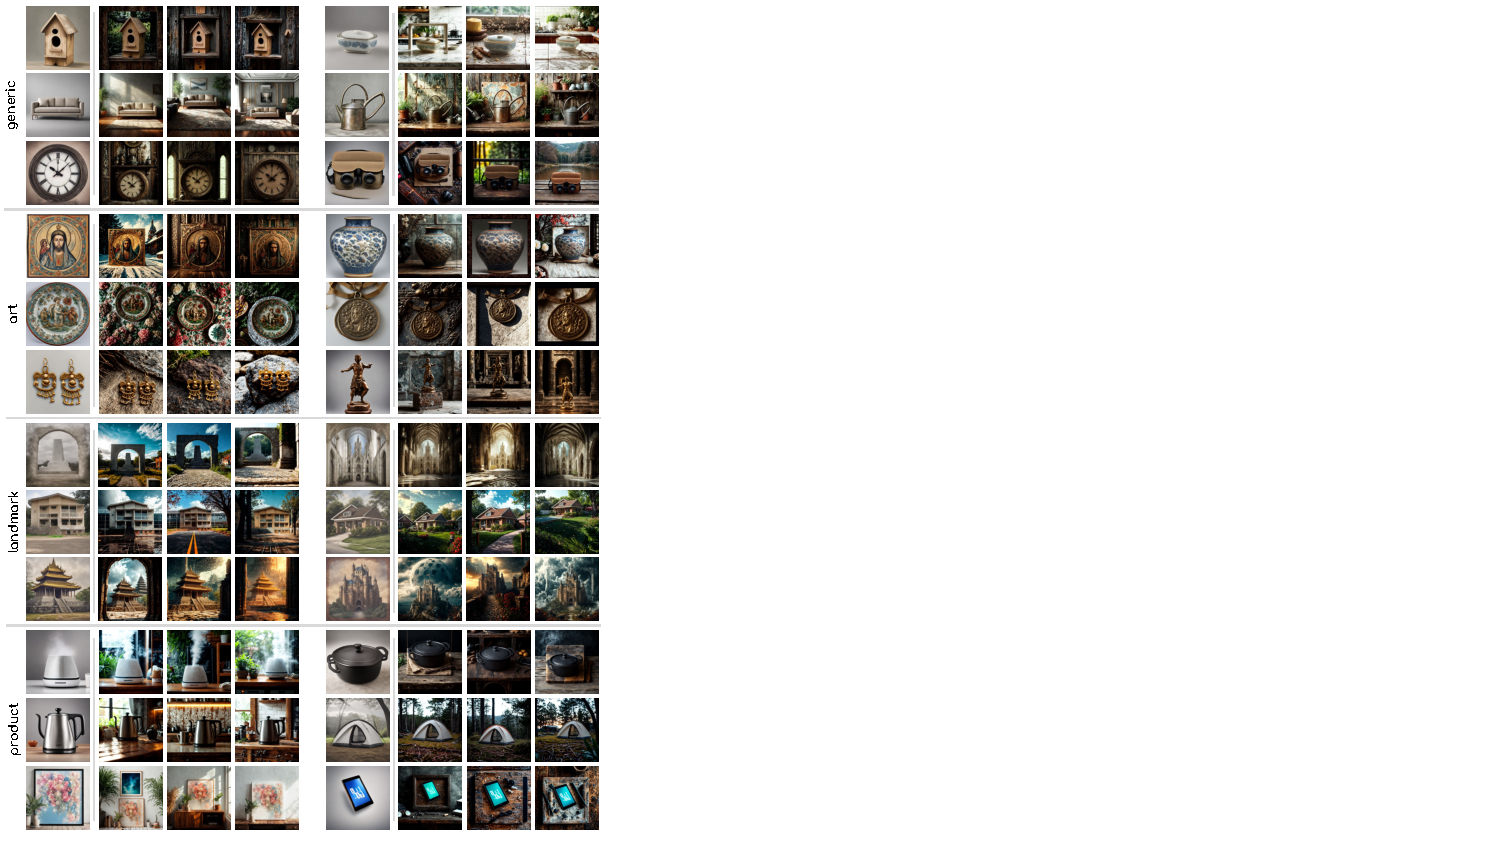
\includegraphics[width=0.91\linewidth]{fig/example.pdf}
\vspace{-9pt}
\caption{Examples of object instances generated by GDM (column 1), and the generated images that leave the object intact and add lighting and background that is well suited to the object (columns 2 $\sim$ 4).
\label{fig:iclight}}
\end{figure*}

\subsection{Representation learning}
%
In total, our generated dataset contains $CKN$ training images, forming $CK$ classes coming from $C$ object categories. 
We construct training batches by sampling $B$ classes and all their corresponding images, resulting in $NB$  images per batch. 
During training, we adopt a query \vs database scheme:
one image from each of the $N$ images per class is randomly chosen as the query, while the remaining $NB-1$ images of the batch form the database, as shown in \cref{fig:batch}.

The similarity between the query and db images is computed in $\hat{\mathbf{y}} \in \mathbb{R}^{NB-1}$, while $\mathbf{y} \in \{0,1\}^{NB-1}$ denotes the labels of all db images with respect to the query, \ie positive or negatives based on their classes. 
We optimize an information retrieval metric as the loss function, in particular an approximation of recall at the top-$k$ ranks, based on $\hat{\mathbf{y}}$, and $\mathbf{y}$.
We train with the average of recall@k loss estimated for different values of $k$.
The approximation of recall is possible by formulating its estimation with the use of step functions, which, during training, are replaced with a sigmoid function.
The technical and implementation details can be found in the original paper~\citep{ptm22}.





\begin{figure}[t]
\begin{center}
\includegraphics[width=0.83\linewidth]{fig/batch.pdf}
\vspace{-10pt}
\caption{Training batch construction for instance-level representation learning. A batch simulates a retrieval task with a query (blue) and database of positive (green) and negative (red) images. Images are considered positive if they belong to the same class, otherwise they are negatives. An image encoder is trained with metric learning on this batch.}
\label{fig:batch}
\end{center}
\end{figure}

\begin{table}[t]
    \centering
    \caption{Statistics of the generated training dataset. \oursgeneric{} and \oursspecific{} comprise only objects from the generic domain and one of the specific domains, respectively.  
    \oursplus{} comprises 50\% of objects from the generic domain ($10$K) and all objects from the three specific domains ($10$K), \ie $20$K objects in total.}
\small
\begin{tabular}{lrrr}
\toprule
\textbf{domain of objects}  & $C$ & $K$ & \textbf{instances} \\ 
\midrule
generic           & $2,000$  & $10$ & $20,000$ \\ 
art        & $200$  & $15$ & $3,000$ \\ 
landmark   & $50$ & $80$  & $4,000$ \\
product    & $200$ & $15$  & $3,000$ \\  
\bottomrule
\end{tabular}

\label{tab:gene_details}
\end{table}

